\subsection{IllustrisTNG}
IllustrisTNG \footnote{https://www.tng-project.org/} is the follow-up project after the success of the Illustris simulations (\textcite{Springel2017}, \textcite{Pillepich2017}, \textcite{Naiman2018}, \textcite{Nelson2017} and \textcite{Marinacci2018}). It is a huge project, built upon a magneto-hydrodynamical cosmological simulation code with added physical processes on a subgrid level \parencite{Weinberger2016}. Adding physical processes like gas radiation, star formation, stellar feedback through supernova explosions, supermassive black hole accretion and magnetic fields are essential to model galaxy formation and evolution and allows a much better comparison to reality. The data output from the simulations is extensive, and is not meant to be analysed all in one go, but rather through a series of analyses, each targeting a specific scientific question. 


\subsubsection{The simulations}
The IllustrisTNG project includes 18 different simulations with varying resolutions, spatial size and included physics. There are three main simulations, TNG300, TNG100 and TNG50, that differ in volume and resolution. The details of these are summed up in Table \ref{TNG}. Each of the main simulations have been run at three different resolution levels, which makes it possible to study how the outcome is affected by changing only the resolution in a given simulation. TNG100 has a physical box volume of $110.7^3 \, $Mpc$^3$, and a baryonic particle resolution of $1.4 \times 10^6 M_{\odot}$, while the TNG300 simulation has a volume of $302.6^3 \, $Mpc$^3$ and a baryonic particle resolution of $1.1 \times 10^7 M_{\odot}$. The TNG50 data is actually not yet available, but it is expected soon, and provides a much higher resolution in a smaller box size. In this project, a large statistical sample of galaxies was needed, as well as detailed structure of the inner part of the galaxies to calculate the different properties, so the TNG100 simulation was the best choice with respect to size and resolution. The TNG100-1 simulation data, which is the highest available resolution for TNG100, has been used throughout the project and will from now on be referenced as TNG only. A visual representation of parts of the simulations can be seen in Figure \ref{tng_illustration}. TNG uses the results from the Planck Collaboration for its cosmology parameters, $\Omega_{\Lambda,0} = 0.6911$, $\Omega_{m,0}=0.3089$, $\Omega_{b,0}=0.0486$, $\sigma_8=0.8159$, $n_s=0.9667$ and $h = 0.6774$ \parencite{Planck2016}. See section \ref{cosmologies} for more details.

\begin{figure}
    \centering
    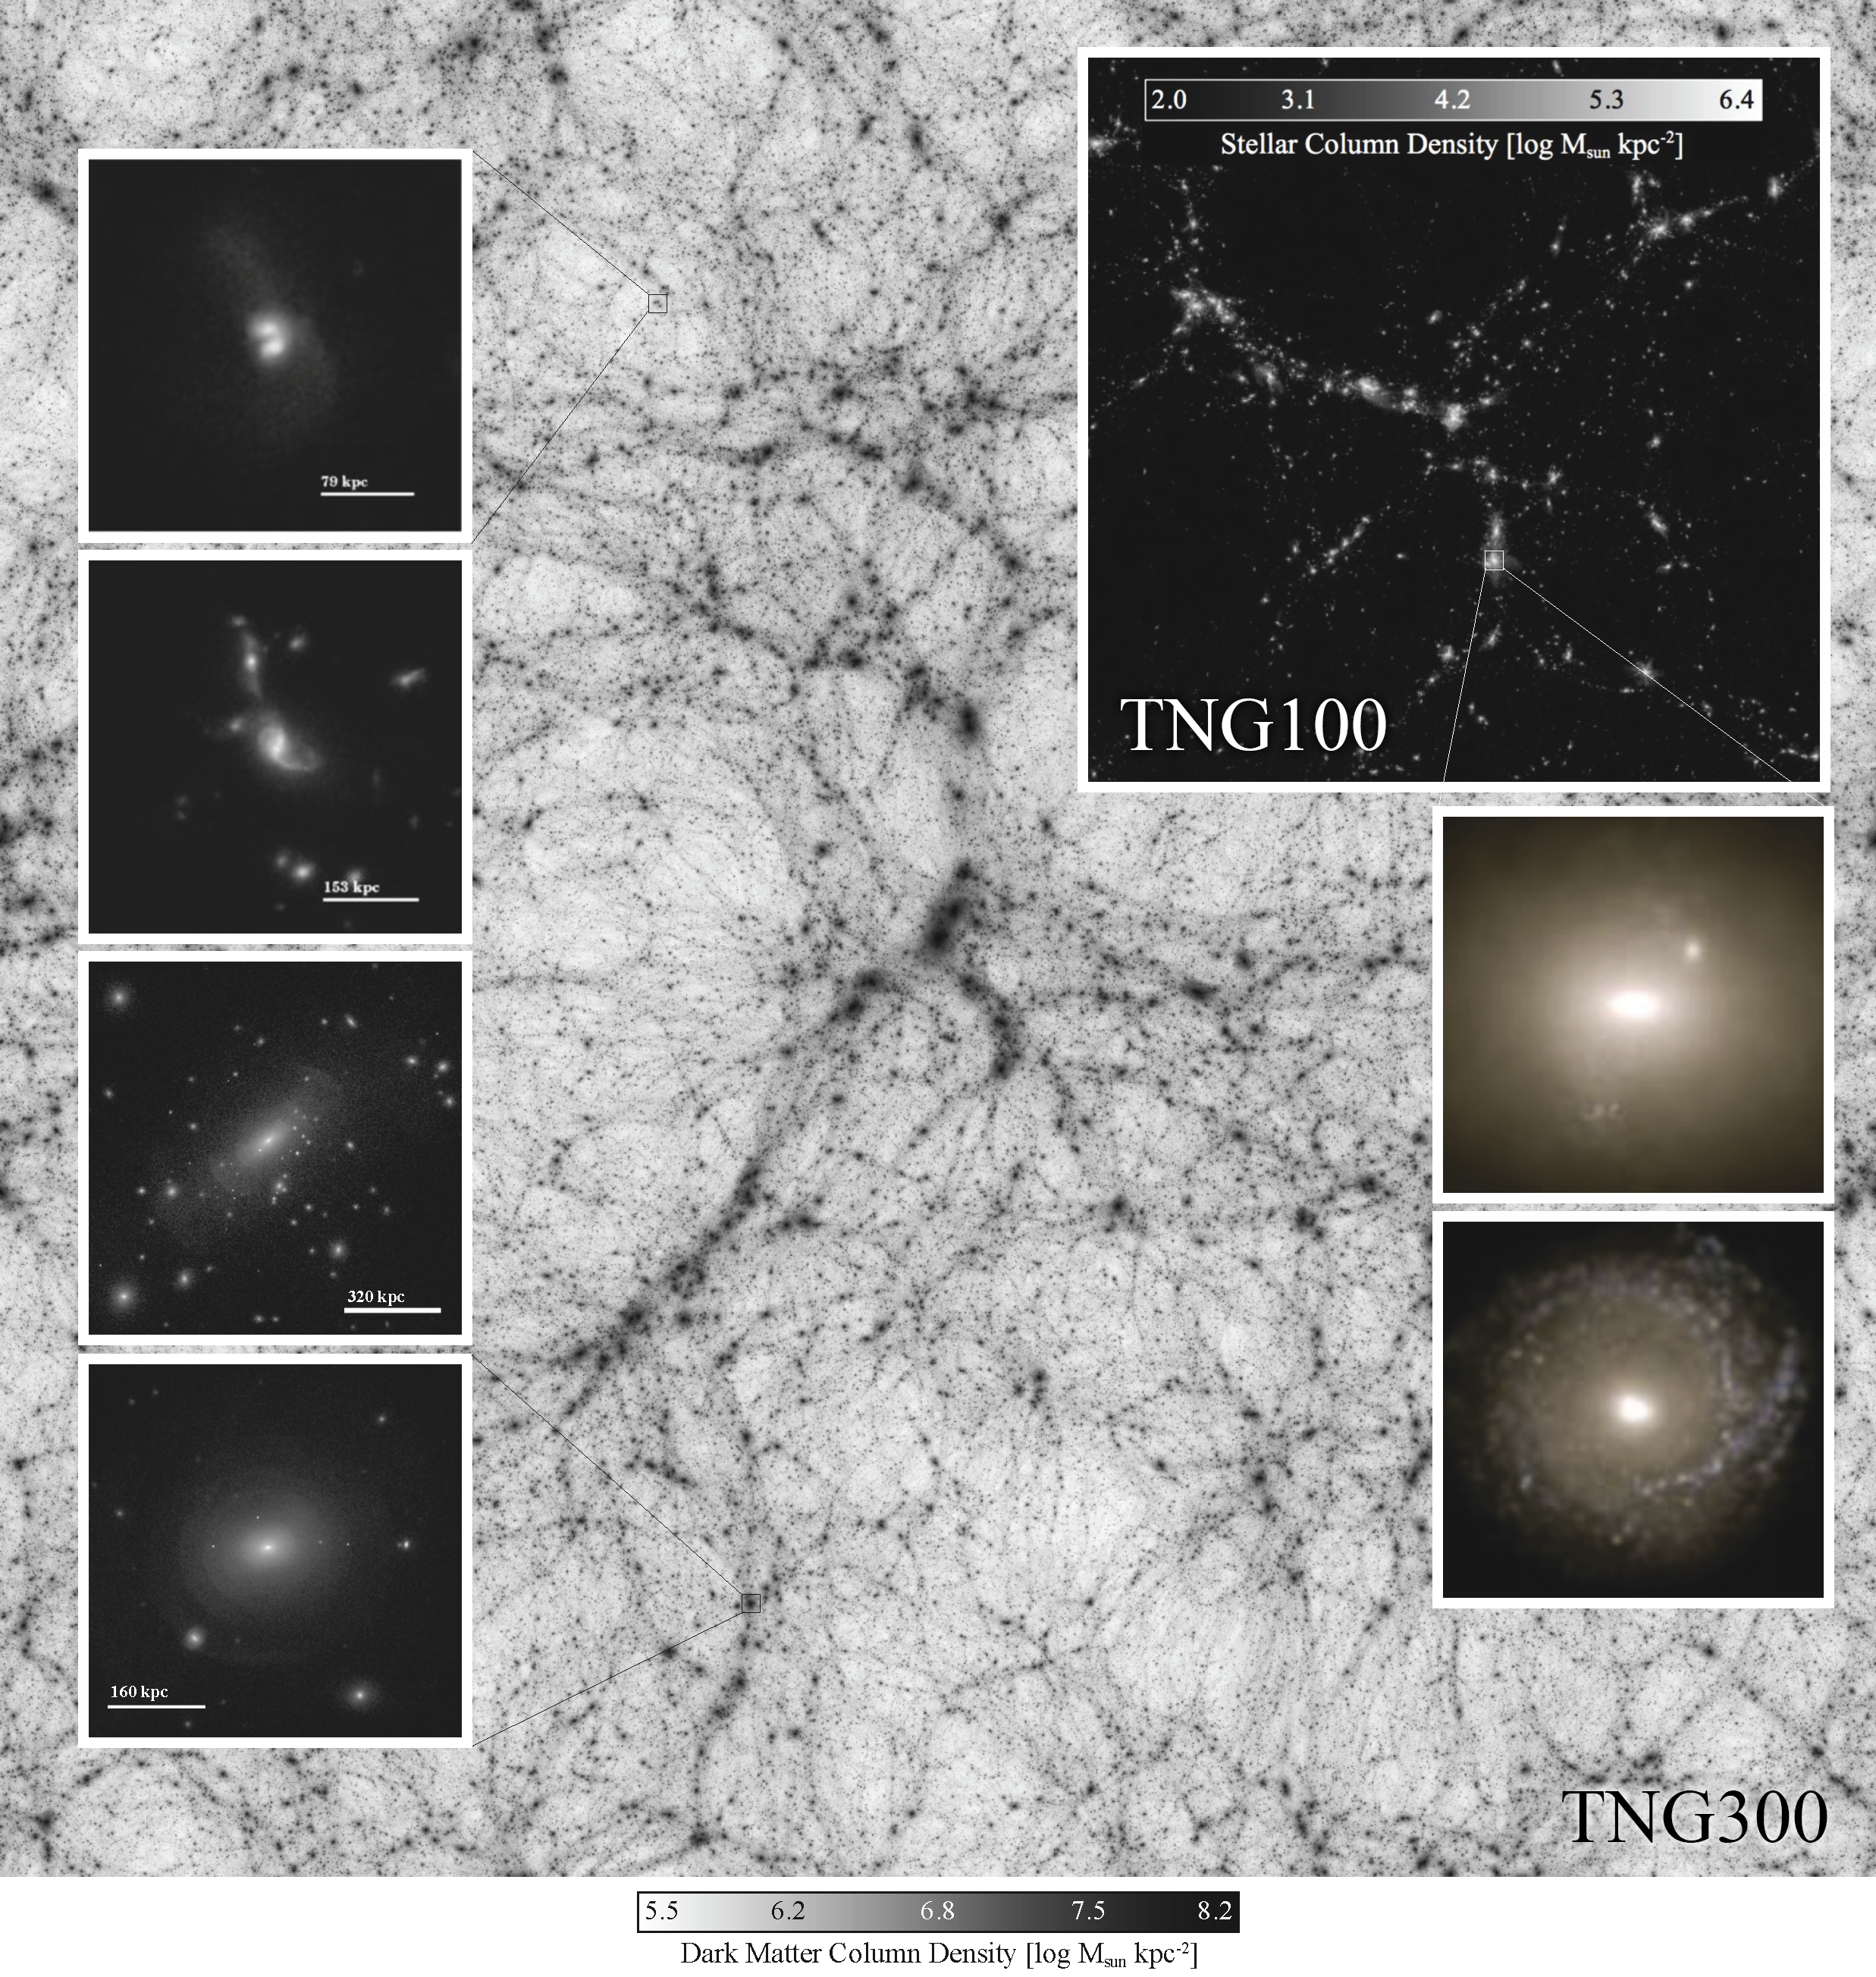
\includegraphics[width=0.9\textwidth]{images/TNG.png}
    \caption{A composite image that illustrates the two simulations TNG100 and TNG300. In the background is the dark matter distribution for the whole TNG300 volume. In the upper right is the stellar mass distribution across the entire TNG100 volume. The panels on the left show galaxy-galaxy interactions, while the panels on the right show the stellar light projections of two $z=0$ galaxies. Credit: TNG Collaboration}.
    \label{tng_illustration}
\end{figure}

\begin{table}
\begin{center}
\caption{The simulation details for the three main TNG simulations. $N_{DM}$ is the amount of dark matter particles. $m_{DM}$ and $m_{baryon}$ is the mass of the dark matter and baryonic particles, respectively.}
 \label{TNG}
\begin{tabular}{ l| c c c c c } 
 \hline
 \hline
   &  Volume [$Mpc^3$] & $N_{DM}$ & $m_{DM}$ [$M_{\odot}$] & $m_{baryon}$ [$M_{\odot}$] \\
 \hline
 TNG50 & $51.7^3$ & $2163^3$ & $4.5 \times 10^5 $ & $8.5 \times 10^4 $ \\ 
 TNG100 & $110.7^3$ & $1820^3$ & $7.5 \times 10^6 $ & $1.4 \times 10^6 $  \\ 
 TNG300 & $302.6^3$ & $2500^3$ & $5.9 \times 10^7 $ & $1.1 \times 10^7 $  \\ 
 \hline 
 \end{tabular}
\end{center}
\end{table}

\subsubsection{Data cataloges}
All the Illustris-TNG data is publically available online at the TNG webpage\footnote{https://www.tng-project.org/data/}. The data products that are available for each simulation are snapshots, group catalogs and merger trees as well as some supplementary data sets. There are five different particle types in the simulations, and each has its properties stored as particle fields. These fields include information like position, kinematic data and atomic/chemical composition. For each different run of the simulation, 100 snapshots are created, which are taken at specific redshifts. They include all the particles in the whole volume of the simulation, with 20 of them including all the fields for each particle as well.

The group catalogs provide a convenient way to quickly access already calculated properties of the different halos and subhalos instead of dealing with all the particles in a snapshot. This saves a lot of time and effort, but gives the user less control over what can be analysed. In future work, it might be interesting to do the calculations directly from the snapshots myself. There is one group catalog for each snapshot, and this includes two types of objects, Friends-of-Friends (FoF) and Subfind. The FoF catalog contains all the halos, and the Subfind catalog contains all the subhalos and their associated galaxy (if there is any) for each halo. Each subhalo has a parent halo, and the largest subhalo in each halo is the central subhalo. The merger trees data products contain the merger history of each subhalo.

This project makes use of the group catalogs for the $z = 0$ snapshot, as we want to compare the output data to observations of the local (present time) Universe.

\subsubsection{Sample reduction}

The TNG documentation recommends filtering out all subhalos that are flagged with the $SubhaloFlag$ field, and so these were cut from the data. These are most probably subhalos of non-cosmological origin, and so should not be considered real galaxies.

For the relations covered in this project, it is desirable to use only the central galaxies in each halo. This is because satellite galaxies are more affected by their environment, which in turn affects the kinematic and structural properties of the galaxy. This will naturally lead to a scatter in the galaxy scaling relations that are being studied, which central galaxies will not display. The FoF catalog contains the index for the largest subhalo in each halo, so combining this information with the Subfind catalog allows one to create a subset of the data that contains only the central galaxies.

Only galaxies with stellar mass greater than $10^9 M_{\odot}$ are used, which corresponds to about 700 stellar particles. Galaxies with fewer particles have less reliably resolved inner structure, and so they are not taken into account for this study.

\subsection{Observational data}
When possible, it is good practice to use the same observational data for comparisons with the simulation data. Trying to accomplish this, in this work I used the SAMI Galaxy Survey \parencite{Bryant2015}. For the SHM relation however, it was not possible to use the SAMI data set, so other works have been chosen to use for that comparison. All the data sets and best fits used in comparing the results from TNG to observations are described in this section.

\subsubsection{SAMI Galaxy Survey}
The Sydney – Australian Astronomical Observatory Multi-Object Integral Field Spectrograph (SAMI) is mounted on the Anglo-Saxan telescope in Australia. The SAMI Galaxy Survey \footnote{https://sami-survey.org/} is a spectroscopic survey of a large sample of galaxies in the nearby Universe ($z < 0.113$). The survey was started in 2013, and ended in 2018. There have been two major data releases, with the newest being Data Release Two (DR2) \parencite{Scott2018}. DR2 includes data for 1559 galaxies, which is about 50 \% of the full galaxy survey. The data products available are IFS data cubes and 2D maps, as well as catalogue data. As the same galaxies have been cataloged in several other studies, data products from those studies are added to SAMI data. Analysing data cubes and 2D maps falls outside the scope of this work, so catalogue data with some properties already estimated is used where possible. 

\subsubsection{Other data sets}
For the SHM relation, best fit models from two different abundance method papers were used in the comparison to TNG.

The first one found a fit to the data by using a power law for the high mass end, and a subpower law for the low mass end \parencite{Behroozi2013}.

\begin{equation} \label{eq_behroozi}
    \log(M_*(M_{halo})) = \log(\epsilon M_1) + f(\log(M_{halo}/M_1)) -f(0),
\end{equation}
\begin{equation*}
    f(x) = -\log(10^{\alpha x}+1)+\delta \frac{(\log(1+\exp(x)))^\gamma}{1 +\exp(10^{-x})}.
\end{equation*}

Here $M_1$ is a characteristic halo mass, $\delta$ is the strength of the subpower law, $\alpha$ is the power law slope for $M_{halo} << M_1$ and $\gamma$ is the power law index for $M_{halo} >> M_1$. The best fit values for the parameters are $M_1 = 11.514\pm(0.053, 0.009)$, $\delta = 3.508 \pm (0.087, -0.369)$, $\alpha = -1.412 \pm (0.020, -0.105)$, $\epsilon = -1.777 \pm (0.133, 0.146)$ and $\gamma = 0.316 \pm (0.076, -0.012)$.

The second one employed the same function for the fit as \textcite{Behroozi2013}, but with different data. The best fit parameters were found to be $M_1 = 11.632\pm(0.008, 0.009)$, $\delta = 3.797 \pm (0.026, 0.021)$, $\alpha = -2.352 \pm (0.026, -0.021)$, $\epsilon = -1.785 \pm (0.010, 0.008)$  and $\gamma = 0.600 \pm (0.10, 0.013)$ \parencite{Zanisi2019}.

\subsection{Morphological classification}
As several of the relations studied in this project relate to the morphological type of the galaxies, it was necessary to filter out early and late type galaxies to study separately. This can be done in different ways. In many studies of TNG, several criteria for classification have been employed at the same time like star formation rate, luminosity profiles, gas fraction and visual classification (see e.g. \textcite{Lu2020} and \textcite{Genel2017}). In this work, the fraction of gas inside the effective radius of each galaxy has been chosen as the single criteria for classification, 

\begin{equation}
    f = M_{gas}/M_*.
\end{equation}

For $f > 0.1$, the galaxy is classified as late type, while for $f< 0.1$, the galaxy is classified as early type. Including a criteria for star formation rate did not significantly change the outcome, so it was determined to keep the selection process simple.

In the SAMI DR2, the galaxy morphology is determined visually. They are classified into four different categories: E, S0, Sa/Sb and Sc/Sd/irregulars, as well as intermediate categories if the gaalaxy is hard to place. See Figure \ref{hubble} in section 2.2 for a visualisation of the different galaxy classifications. In this analysis, the E and S0 are considered early type, while Sa/Sb and Sc/Sd/irregulars are considered late types.

\subsection{Calculating properties}

\subsubsection{Cosmologies and h-dependence} \label{cosmologies}
When making measurements of galaxy properties, some assumptions about the underlying cosmology of the Universe must be made. One of these assumptions is the value of the Hubble constant $H_0$, more commonly represented by $h$, where $H_0 = 100\,h\,$ km/s/Mpc. In addition to several other cosmological parameters, this constant is used when running a cosmological simulation. Astrophysical properties, both numerical and observational, are presented in publications with an h-dependence (leaving the user to specifiy the cosmology) or without an h-dependence (by assuming a value for h).

For IllustrisTNG, $h=0.6774$ and the explicit $h$-dependence of each property value is stated clearly in the documentation. For the SAMI data catalogue, no $h$-dependence is explicitly stated in the documentation or data release papers, but the Hubble constant used is given as $h = 0.7$.

Best practice dictates that to compare works with different assumed Hubble constants, the $h$ used in those specific works should be replaced with the most recent value for $h$ \parencite{Croton2013}. The values for galaxy properties will then be comparable. In Table \ref{h_dependence} the h-dependency of the galaxy properties of TNG as well as the common h-dependencies for observational data is shown along with their corresponding units. In this work, all data results are converted to the TNG cosmology, which uses the newest values for the cosmological parameters.

\begin{table}
\begin{center}
\caption{The $h$-dependence and units for the galaxy properties used in this work. For TNG, the dependency is given in the data documentation. The dependencies for SAMI are the standard dependencies for observational data, as found in Table 2 in \textcite{Croton2013}.}
\label{h_dependence}
\begin{tabular}{ l| c c }
 \hline
 \hline
   & TNG & SAMI \\
 \hline
 Stellar mass & $M_{\odot}h^{-1}$ & $M_{\odot}h^{-2}$ \\ 
 Halo mass & $M_{\odot}h^{-1}$ & - \\
 Size & kpc$\,h^{-1}$ & kpc$\,h^{-1}$ \\
 Luminosity & mag & mag $+5\log(h)$ \\
 Velocity & km/s & km/s  \\ 

 \hline 
\end{tabular}
\end{center}
\end{table}


\subsubsection{Magnitude and colors}
The magnitude ($\mathcal{M}$) is a measure of the total luminosity ($L$) of the galaxy such that $\mathcal{M} = -2.5 \log(L/L_\odot) + \mathcal{M}_\odot$, where $L_\odot$ is the solar luminosity and $\mathcal{M}_\odot$ is the solar magnitude.

For the TNG data, the Subhalo field \texttt{SubhaloStellarPhotometrics} is used to get the magnitudes based on the summed up luminosities of all the stellar particles in the Subhalo. Eight bands are available, but in this work only the g- and i-band are used. The g-i colors are calculated by simply subtracting the i-band magnitude from the g-band magnitude.

In SAMI, g-i color values are adopted from the GAMA Sérsic catalogue \parencite{Driver2011}.

\subsubsection{Stellar mass}
The stellar mass of each galaxy in both TNG and SAMI are readily available in the group catalogs. Stellar mass estimates depend on the stellar initial mass function (IMF), which describe the spectral evolution of a population of stars, and as such the relationship between luminosity and mass in a given spectral band. SAMI and TNG both adopt a \textcite{Chabrier2003} IMF.

For SAMI DR2, the stellar mass values are taken from the GAMA Sérsic catalogue \parencite{Driver2011}. They calculate the stellar masses by using the i-band magnitude and g-i color of each galaxy through the formula $\log M_*/M_\odot = 1.15 + 0.70(g-i) -0.4\mathcal{M}_i$, where $\mathcal{M}_i$ is the rest-frame i-band absolute magnitude \parencite{Taylor2011}.

\subsubsection{Size}\label{radius}
In observational data, galaxy sizes are always projected sizes, as they are derived from 2D images. A common measure of the size of a galaxy is the effective radius, which is the radius within which half the light of the galaxy is contained. This quantity depends on the analysis and quality of the 2D profiles, and may not be able to include all the light in a galaxy in the way that we can ensure for computer simulated data. The radius also depends on which optical filter the measurements are made in, as different filters will capture different parts of the galaxy.

For TNG data, the \texttt{SubhaloHalfmassRadStellar} field has been used. The half-mass radius is the radius of a spherical volume within which half the stellar mass is found. It is the 3D half-mass radius ($R_e$), as it is not a projected quantity. This value is generally higher than the 2D half-light radius ($r_e$) for a given mass up to $M_{*} < 10^{10.5}$, as seen in \textcite{Genel2017}. To be consistent with observed data, the 3D radius is projected by using the relation $R_{e} = \frac{4}{3}r_{e}$ which generally holds for pressure supported systems like elliptical galaxies \parencite{Wolf2010}.

The SAMI catalog data takes the values for the effective radius from the GAMA Sérsic catalogue \parencite{Driver2011}. The effective radius is defined as the semi-major axis half-light radius, measured in the r-band. The values are given in units of arcsec which were then converted to a physical radius in kpc.

Then these semi-major axis radii are converted to circular radii using the formula

\begin{equation}
   r_{e, circ} = r_{e, sm}\sqrt{(1-\epsilon)},
\end{equation}

where $r_{e, circ}$ is the circular radius, $r_{e,sm}$ is the semi-major axis effective radius and $\epsilon$ is the eccentricity.

\subsubsection{Velocities}

Galaxy velocities are for early and late type galaxies are usually defined as respectively velocity dispersion and rotational velocity. This is because of the shape of the two different galaxy types. It makes more sense to talk about velocity dispersion in a pressure dominated system and rotational velocity in a rotating disk.

For the TFR, rotational velocities are needed. In TNG, the Subhalo field \texttt{SubhaloVMax} gives the maximum value for the spherically averaged rotation curve of a given galaxy. As the rotational curves are nearly flat for large enough radii, it should not be very important at which radius the observational rotational velocity is measured, as long as it is in the flat part of the curve. Accordingly, \texttt{SubhaloVMax} is used as the rotational velocity for the TNG data.

Rotational velocities were not available as SAMI catalogue data, but an extensive analysis of the 2D velocity maps in DR2 is found in \textcite{Bloom2017}. They defined the rotational velocity as the velocity at $2.2\, R_e$, which should lay well into the flat regime of the velocity curve, and coincide well with the maximum velocity. Their best fit for the TFR was used in our comparison, 
\begin{equation}
	\log(V_{rot}) = 0.31 \pm 0.0092 \times \log(M_*)-0.93 \pm 0.1.
\end{equation}

When talking about the FJ relation and the fundamental plane, velocity dispersion is the velocity measure which is used. The field \texttt{SubhaloVelDisp} from the TNG group catalog gives the velocity dispersion of all the member particles for each subhalo. In SAMI catalog data, the given velocity dispersion is averaged within an aperture with radius equal to the effective radius of each galaxy.